\documentclass[sigconf]{acmart}

\setlength{\paperheight}{11in}
\setlength{\paperwidth}{8.5in}

\usepackage[utf8]{inputenc}

\hyphenation{regarding}

\usepackage{amsmath,amssymb}
%\usepackage{amsthmnoproof}
\usepackage{amsthm}
\usepackage{mathrsfs}
%\let\bibsection\relax
%\usepackage{amsrefs}
%\usepackage[usenames,dvipsnames]{color}
\usepackage{stmaryrd}
\usepackage{enumerate}
%\usepackage[algoruled,vlined,english,linesnumbered]{algorithm2e}
%\usepackage[pdfpagelabels,colorlinks=true,citecolor=blue]{hyperref}
\usepackage{comment}
\usepackage{multirow}
\usepackage{xspace}
\usepackage{tabularx,multicol}
\usepackage{tikz}

\newcommand{\noopsort}[1]{}
\DeclareMathOperator{\NP}{NP}
\DeclareMathOperator{\HP}{HP}
\DeclareMathOperator{\PP}{PP}
\DeclareMathOperator{\Hom}{Hom}
\DeclareMathOperator{\End}{End}
\DeclareMathOperator{\GL}{GL}
\DeclareMathOperator{\val}{val}
\DeclareMathOperator{\pr}{pr}
\DeclareMathOperator{\tr}{Tr}
\DeclareMathOperator{\adj}{Adj}
\DeclareMathOperator{\Grass}{Grass}
\DeclareMathOperator{\Lat}{Lat}
\DeclareMathOperator{\round}{round}
\DeclareMathOperator{\rank}{rank}
\DeclareMathOperator{\lcm}{lcm}
\DeclareMathOperator{\rec}{rec}
\DeclareMathOperator{\cond}{cond}
\DeclareMathOperator{\disc}{Disc}
\DeclareMathOperator{\row}{row}
\DeclareMathOperator{\col}{col}

\newcommand{\ph}{\vphantom{$A^A_A$}}

\newcommand{\N}{\mathbb N}
\newcommand{\Z}{\mathbb Z}
\newcommand{\Zp}{\Z_p}
\newcommand{\Q}{\mathbb Q}
\newcommand{\Qp}{\Q_p}
\newcommand{\Fp}{\mathbb{F}_p}
\newcommand{\Fq}{\mathbb{F}_q}
\newcommand{\R}{\mathbb R}
\newcommand{\OK}{\mathcal{O}_K}

\newcommand{\calV}{\mathcal{V}}
\newcommand{\ttv}{\texttt{v}\xspace}
\newcommand{\ttw}{\texttt{w}\xspace}
\newcommand{\tttmp}{\texttt{tmp}\xspace}
\newcommand{\calU}{\mathcal{U}}
\newcommand{\calK}{\mathcal{K}}

\newcommand{\rem}{\,\%\,}

\newcommand{\sage}{\textsc{SageMath}\xspace}
\newcommand{\ZpL}{\text{\rm \tt ZpL}\xspace}
\newcommand{\ZpLC}{\text{\rm \tt ZpLC}\xspace}
\newcommand{\ZpLF}{\text{\rm \tt ZpLF}\xspace}

\newcommand{\card}{\text{Card}\:}
\newcommand{\ind}{\text{ind}}
\newcommand{\coind}{\text{coind}}

\newcommand{\famN}{\mathcal{N}}

\newcommand{\llb}{[\mkern-2.5mu[}
\newcommand{\rrb}{]\mkern-2.5mu]}
\newcommand{\llp}{(\mkern-2.5mu(}
\newcommand{\rrp}{)\mkern-2.5mu)}


\newcommand{\softO}{O\tilde{~}}

\newcommand{\inv}{\text{\rm inv}}
\newcommand{\app}{\text{\rm app}}

\newcommand{\cIn}{{\color{blue} \tt \phantom{Zp}In}:}
\newcommand{\cOut}{{\color{red} \tt \phantom{Z}Out}:}
\newcommand{\cZpCR}{{\color{red} \tt ZpCR}:}
\newcommand{\cZpFP}{{\color{red} \tt ZpFP}:}
\newcommand{\cZpLC}{{\color{red} \tt ZpLC}:}
\newcommand{\cZpLF}{{\color{red} \tt ZpLF}:}

\def\todo#1{\ \!\!{\color{red} #1}}
\definecolor{purple}{rgb}{0.6,0,0.6}
\def\todofor#1#2{\ \!\!{\color{purple} {\bf #1}: #2}}

\newcommand{\done}[1]{\textcolor{blue}{#1}}
\newcommand{\tdo}[1]{\textcolor{red}{#1}}
\definecolor{answer}{rgb}{0,0.5,0.2}
\newcommand{\xavier}[1]{\textcolor{answer}{{\bf Xavier:} #1}}
\newcommand{\tristan}[1]{\textcolor{answer}{{\bf Tristan:} #1}}
\newcommand{\david}[1]{\textcolor{answer}{{\bf David:} #1}}

\def\binom#1#2{\Big(\begin{array}{cc} #1 \\ #2 \end{array}\Big)}

\clubpenalty=10000
\widowpenalty = 10000

\newtheorem{theo}{Theorem}[section]
\newtheorem{lem}[theo]{Lemma}
\newtheorem{prop}[theo]{Proposition}
\newtheorem{cor}[theo]{Corollary}
\newtheorem{quest}[theo]{Question}
\newtheorem{conj}[theo]{Conjecture}
\theoremstyle{definition}
\newtheorem{rmk}[theo]{Remark}
\newtheorem{ex}[theo]{Example}
\newtheorem{deftn}[theo]{Definition}

\fancyhead{}

\begin{document}

\title{\ZpL: a p-adic precision package}

\author{Xavier Caruso}
  \affiliation{Universit\'e Rennes 1; \\
  \institution{IRMAR}
  \city{Rennes, France}
  \postcode{35042}
}
\email{xavier.caruso@normalesup.org}
\author{David Roe}
  \affiliation{University of Pittsburg; \\
  \institution{Department of Mathematics}
  \city{Pittsburgh, PA, USA}
  \postcode{15260}
}
\email{roed@pitt.edu}
\author{Tristan Vaccon}
  \affiliation{Universit\'e de Limoges; \\
  \institution{CNRS, XLIM UMR 7252}
  \city{Limoges, France}  
  \postcode{87060}  
  }
\email{tristan.vaccon@unilim.fr}

\ccsdesc[500]{Computing methodologies~Algebraic algorithms}

\keywords{Algorithms, $p$-adic precision, Automatic Differentiation}

\begin{abstract}
We present a new package \ZpL for the Computer Algebra system \sage. It 
implements a sharp tracking of precision on $p$-adic numbers, following 
the theory of ultrametric precision introduced in \cite{padicprec}. The 
underlying algorithms are mostly based on Automatic Differentiation 
techniques. We introduce them, study their complexity and discuss our 
design choices.
We illustrate the benefits of our package (in comparison with previous 
implementations) with a large sample of examples coming from Linear 
Algebra, Commutative Algebra and Differential Equations.
\end{abstract}

\maketitle

\section{Introduction}

\begin{itemize}
\item Interval arithmetic, floating point arithmetic
\item short introduction of the precision lemma and lattices
\item goal: tracking precision using this theory
\item short presentation of the package
\item plan of the article
\end{itemize}

\todo{Convention: in matrices, vectors are represented by row-vector.}

\section{Examples}

\subsection{Elementary arithmetic}

\begin{tabular}{|l|l|}
\verb?R = Zp(3,5)? & \verb?R = ZpL(3,5)? \\
\verb?x = R(143,5); x? & \verb?x = R(143,5); x? \\
\hfill\verb?...12022? & \hfill\verb?...12022? \\
\verb?3*x? & \verb?3*x? \\
\hfill\verb?...120220? & \hfill\verb?...120220? \\
\verb?x + x + x? & \verb?x + x + x? \\
\hfill\verb?...20220? & \hfill\verb?...120220? \\
\verb?x^3? & \verb?x^3? \\
\hfill\verb?...020222? & \hfill\verb?...020222? \\
\verb?x * x * x? & \verb?x * x * x? \\
\hfill\verb?...20222? & \hfill\verb?...020222? \\
\end{tabular}

\begin{tabular}{|l|l|}
\verb?R = Zp(2,10)? & \verb?R = ZpL(2,10)? \\
\verb?x = R(987,10); x? & \verb?x = R(987,10); x? \\
\hfill\verb?...1111011011? & \hfill\verb?...1111011011? \\
\verb?y = R(21,5); y? & \verb?y = R(21,5); y? \\
\hfill\verb?...10101? & \hfill\verb?...10101? \\
\verb?u = x + y; u? & \verb?u = x + y; u? \\
\hfill\verb?...10000? & \hfill\verb?...10000? \\
\verb?v = x - y; v? & \verb?v = x - y; v? \\
\hfill\verb?...00110? & \hfill\verb?...00110? \\
\verb?u + v? & \verb?u + v? \\
\hfill\verb?...10110? & \hfill\verb?...11110110110? \\
\end{tabular}

\subsection{Linear algebra}

\begin{itemize}
\item determinant
\item characteristic polynomial
\end{itemize}

\subsection{Commutative algebra}

\begin{itemize}
\item gcd of polynomials
\end{itemize}

\section{Presentation of the package}

In this Section, we explain how our package \ZpL works and analyze
its performances.
The main theoretical result on which our package is based in the 
ultrametric precision theory developed in \cite{padicprec}, which 
suggests to track precision \emph{via} lattices and differential 
computations. For this reason, our approach is very inspired by 
Automatic Differentiation techniques \cite{} and our implementation 
follows the usual Operator Overloading strategy \cite{}.
We will introduce two versions of our package, namely \ZpLC and \ZpLF: 
this former is safer while the latter is faster.

This Section is organized as follows.
\todo{[...]}.

\smallskip

\noindent \textit{Remark about the naming.}
%
The letter \texttt{L}, which appears in the name of the package, 
comes from ``lattices''. The letters \texttt{C} (in \ZpLC) and 
\texttt{F} (in \ZpLF) stand for ``cap'' and ``float'' respectively.

\subsection{The precision Lemma}
\label{ssec:preclemma}

In \cite{caruso-roe-vaccon:14a}, we have suggested the 
use of lattices to represent the precision of elements in 
$K$-vector spaces.  It contrasts with the
\emph{coordinate-wise method} (of \textit{e.g.}
 \verb?Zp(5)?) that is used traditionally in \sage and
where the precision of an element is specified by giving the precision
of each coordinate separately and is updated after each basic
operation.

Consider a finite 
dimensional normed vector space $E$ 
defined over $K$. 
We use the notation $\Vert \cdot \Vert_E$ for the norm 
on $E$ and $B^-_E(r)$ (resp. $B^{\phantom -}_E(r)$) for the open (resp. 
closed) ball of radius $r$ centered at the origin. A \emph{lattice} $L \subset 
E$ is a sub-$\O_K$-module which generates $E$ over $K$. 
Because of ultrametricity, the balls $B^{\phantom 
-}_E(r)$ and $B^-_E(r)$ are examples of lattices. 
Lattices can be thought of as special neighborhoods of $0,$
 and therefore are good 
candidates to model precision data. Moreover, as revealed in 
\cite{caruso-roe-vaccon:14a}, they behave quite well under (strictly) 
differentiable maps:

\begin{prop}
\label{prop:precision}
Let $E$ and $F$ be two finite dimensional normed vector spaces over $K$ 
and $f : U \rightarrow F$ be a function defined on an open subset $U$ of 
$E$. We assume that $f$ is differentiable at some point $v_0 \in U$ and 
that the differential $df_{v_0}$ is surjective.
Then, for all $\rho \in (0, 1]$, there exists a positive real
number $\delta$ such that, for all $r \in (0, \delta)$, any lattice
$H$ such that $B^-_E(\rho r) \subset H \subset B^{\phantom -}_E(r)$ 
satisfies:
\begin{equation}
\label{eq:firstorder}
f(v_0 + H) = f(v_0) + df_{v_0} (H).
\end{equation}
\end{prop}

This proposition enables the \emph{lattice method} of tracking precision,
where the precision of the input is specified as a lattice $H$ and precision
is tracked via differentials of the steps within a given algorithm.
The equality sign in Eq.~\eqref{eq:firstorder} shows that this method
yields the optimum possible precision. 
We refer to \cite[\S 4.1]{caruso-roe-vaccon:14a} for a more complete 
exposition.
We emphasize that polynomials, rational fractions (outside of their poles)
and converging power series are strictly differentiable.

The lemma is more precise in the context of so-called
integral polynomial functions.
A function $f : E \to F$ is said to be
\emph{integral polynomial} if it is given by multivariate polynomial 
functions with coefficients in $\O_K$ in any (equivalently all) system 
of coordinates associated to a $\OK$-basis of $B_E(1)$.

\begin{prop}
\label{prop:precision2}
We keep the notation of Proposition \ref{prop:precision} and assume 
in addition that $f$ is integral polynomial. Let $C$ be a positive real
number such that $B_F(1) \subset df_{v_0}(B_E(C))$. 
Then Proposition \ref{prop:precision} holds with $\delta = C \cdot
\rho^{-1}$.
\end{prop}

We will use the following definition to measure the gap
between lattice and coordinate-wise methods. 
Suppose $E$ is equipped with a basis $(e_1, \ldots, e_n)$ and write $\pi_i : E \to Ke_i$ for the projections.

\begin{deftn} \label{def:diffused}
Let $H \subset E$ be a lattice. The number of 
\emph{diffused digits of precision} of $H$ is the length of
$H_0/H$ where $H_0 = \pi_1(H) \oplus \cdots \oplus \pi_n(H)$.
\end{deftn}
If $H$ represents the actual precision on some object, then
$H_0$ is the smallest diagonal lattice containing $H$.
Coordinate-wise methods, with one precision datum per coordinate,
corresponds to diagonal lattices.
Hence, they cannot yield a precision better than $H_0$, and
then $k$ provides a lower bound on the number of $p$-adic digits
gained by lattice methods over standard methods.

\subsection{Tracking precision}

\todo{Maybe, add a short intro.}

In what follows, it will be convenient to use a notion of discrete time 
represented by the letter $t$. Rigorously, it is defined as follows: 
$t=0$ when the $p$-adic ring $\ZpLC(\:\cdots)$ is created and increases by 
$1$ each time a variable is created, deleted\footnote{The deletion can
be explicit (through a call to the \texttt{del} operator) or implicit
(handled by the garbage collector).} or updated.

Let $\calV_t$ be the set of alive variables at time $t$. Set $E_t = 
\Qp^{\calV_t}$; it is a finite dimensional vector space over $\Qp$ which 
should be thought as the set of all possible values that can be taken by 
the variables in $\calV_t$. For $\ttv \in \calV_t$, let $e_\ttv \in
\Qp^{\calV_t}$ be the vector whose all coordinates vanished except 
that at position $\ttv$ which takes the value $1$. The family 
$(e_\ttv)_{\ttv \in \calV_t}$ is obviously a basis of $E_t$; we will 
refer to it as the \emph{canonical basis}.

\subsubsection{The case of \ZpLC.}

Following Proposition~\ref{prop:precision},
the package \ZpLC follows the precision by keeping track of a lattice
$H_t$ in $E_t$, which is a global object whose purpose is to model the 
precision on all the variables in $\calV_t$ all together.
Concretely, this lattice is represented by a matrix $M_t$ in row-echelon 
form whose rows form a set of generators.
Below, we explain how the matrices $M_t$ are updated each time
$t$ increases.

\smallskip

\noindent \textit{Creating a variable.}
%
This happens when we encounter an instruction having one of the
two following forms:

\medskip

\noindent \hspace{5mm} \makebox[2.5cm]{[Computation]\hfill\null}
\verb?w = ?$f$\verb?(v_1,? \ldots\verb?, v_n)?

\smallskip

\noindent \hspace{5mm} \makebox[2.5cm]{[New value]\hfill\null}
\verb?w = ?\verb?R(?\text{value}\verb?, ?\text{prec}\verb?)?

\medskip

\noindent
In both cases, $\ttw$ is the newly created variable. 
The $\ttv_i$'s stand for already defined variables and $f$ is some 
$n$-ary builtin function (in most cases it is just addition, 
subtraction, multiplication or division). On the contrary, the terms 
``value'' and ``prec'' refer to user-specified constants or integral 
values which was computed earlier.

\smallskip

Let us first examine the first construction [Computation].
With our conventions, if $t$ is the time just before the execution of 
the instruction we are interested in, the $\ttv_i$'s lie in $\calV_t$ 
while $\ttw$ does not. Moreover $\calV_{t+1} = \calV_t \sqcup \{\ttw\}$, 
so that $E_{t+1} = E_t \oplus \Qp e_\ttw$.
The mapping taking the values of variables at time $t$ to that at 
time $t{+}1$ is:
$$\begin{array}{rcl}
F: \quad E_t & \longrightarrow & E_{t+1} \smallskip \\
\underline x & \mapsto & \underline x \:\oplus f(x_1, \ldots, x_n)
\end{array}$$
where $x_i$ is the $\ttv_i$-th coordinate of the vector $\underline x$.
The Jacobian matrix of $F$ at $\underline x$ is easily computed; it 
is the block matrix $J_{\underline x}(F) = \big( \begin{matrix} I & L
\end{matrix} \big)$ where $I$ is the identity matrix of size $\text{Card}
\:\calV_t$ and $L$ is the column vector whose $\ttv$-th entry is
$\frac{\partial f}{\partial \ttv} (\underline x)$ if $\ttv$ is one of 
the $\ttv_i$'s and $0$ otherwise.
Therefore, the image of $H_t$ under $dF_{\underline x}$ is represented 
by the matrix $J_{\underline x}(F) \cdot M_t = \big( \begin{matrix} M_t & C
\end{matrix} \big)$ where $C$ is the column vector:
$$C = \sum_{i=1}^n \frac{\partial f}{\partial{\ttv_i}} (\underline x)
\cdot C_i$$
where $C_i$ is the column vector of $M_t$ corresponding to the
variable $\ttv_i$.
Observe that the matrix $J_{\underline x}(F) \cdot M_t$ is no longer a 
square matrix; it has one extra column. This reflects the fact that 
$\dim E_{t+1} = \dim E_t + 1$. Rephasing this in a different language, 
the image of $H_t$ under $dF_{\underline x}$ is no longer a lattice in 
$E_{t+1}$ but is included in an hyperplane.

The package \ZpLC tackles this issue by introducing a cap: we do not 
work with $dF_{\underline x}(H_t)$ but instead define the lattice: 
$$H_{t+1} = dF_{\underline x}(H_t) \oplus p^{N_{t+1}} \Zp e_\ttw$$
where $N_{t+1}$ is an integer, the so-called \emph{cap}.
Alternatively, one may introduce the application:
\begin{equation}
\label{eq:tildeF}
\begin{array}{rcl}
\tilde F: \quad E_t \oplus \Qp & \longrightarrow & E_{t+1} \smallskip \\
\underline x \oplus c & \mapsto & \underline x \:\oplus 
\big(f(x_1, \ldots, x_n) + c\big).
\end{array}
\end{equation}
The lattice $H_{t+1}$ is then the image of $H_t \oplus p^{N_{t+1}}
\Zp$ under $d\tilde F_{(\underline x, \star)}$ for any value of $\star$.
The choice of the 
cap is of course a sensitive question. \ZpLC proceeds as follows. When a 
ring is created, it comes with two constants (which can be specified by 
the user): a relative cap \textsc{relcap} and an absolute cap 
\textsc{abscap}. With these predefined values, the chosen cap is:
\begin{equation}
\label{eq:cap}
N_{t+1} = 
\min\big(\textsc{abscap},\, \textsc{relcap} + v_p(y)\big)
\end{equation}
with $y = f(x_1, \ldots, x_n)$.

In concrete terms, the lattice $H_{t+1}$ is represented by the block 
matrix:
$$\left(\begin{matrix}
M_t & C \smallskip \\ 0 & p^{N_{t+1}}
\end{matrix}\right).$$
Performing row operations, we see then the entries of $C$ can be
reduced modulo $p^{N_{t+1}}$ without changing the lattice. In order
to optimize the size of the objects, we perform this reduction and
define $M_{t+1}$ by:
$$M_{t+1} = \left(\begin{matrix}
M_t & C \text{ mod } p^{N_{t+1}} \smallskip \\ 0 & p^{N_{t+1}}
\end{matrix}\right).$$
We observe in particular that $M_{t+1}$ is still in row-echelon form.

Finally, we need to precise which value is set to the newly created 
variable $\ttw$. We observe that it cannot be exactly $f(x_1, \ldots, 
x_n)$ because the latter is \emph{a priori} a $p$-adic number which 
cannot be computed exactly. For this reason, we have to truncate it at 
some finite precision. Again we choose the precision $O(p^{N_{t+1}})$,
\emph{i.e.} we define $x_\ttw$ as $f(x_1, \ldots, x_n) \text{ mod } 
p^{N_{t+1}}$. This makes sense because:
$$\bar x \oplus f(x_1, \ldots, x_n) \equiv
\bar x \oplus x_\ttw \pmod{H_{t+1}}$$
thanks to the extra generator we have added.

\smallskip

The second construction
``\verb?w = ?\verb?R(?\text{value}\verb?, ?\text{prec}\verb?)?''
is easier to handle since, roughly speaking, it corresponds to the
case $n = 0$.
In this situation, keeping in mind the cap, the lattice $H_{t+1}$ is 
defined by:
$$H_{t+1} = H_t + p^{\min(\text{prec}, N_{t+1})} \Zp e_\ttw$$
where the cap $N_{t+1}$ is:
$$N_{t+1} = \min\big(\textsc{abscap},\, \textsc{relcap} + 
v_p(\text{value})\big).$$
The corresponding matrix $M_{t+1}$ is then given by:
$$M_{t+1} = \left(\begin{matrix}
M_t & 0 \smallskip \\ 0 & p^{\min(\text{prec}, N_{t+1})}
\end{matrix}\right).$$


\medskip

\noindent \textit{Deleting a variable.}
%
Let us now examine the case where a variable $\ttw$ is deleted (or 
collected by the garbage collector). Just after the deletion, at
time $t{+}1$, we then have $\calV_{t+1} = \calV_t \backslash \{\ttw\}$.
Thus $E_t = E_{t+1} \oplus \Qp e_\ttw$. Moreover, the deletion of $\ttw$
is modeled by the canonical projection $f : E_t \to E_{t+1}$. Since $f$
is linear, it is its own differential (at each point) and we set 
$H_{t+1} = f(H_t)$.
A matrix representing $H_{t+1}$ is deduced from $M_t$ by erasing the 
column corresponding to $\ttw$. However the matrix we get this way is 
no longer in row-echelon form. We then need to re-echelonize it.

\smallskip

More precisely, in the \ZpLC case, the obtained matrix has this 
shape:
$$\left(\raisebox{-0.5\height}{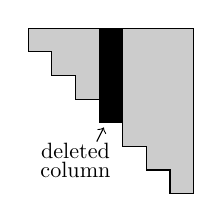
\begin{tikzpicture}[scale=0.3]
\fill[black!20] (0,0)--(0,-1)--(1,-1)--(1,-2)--(2,-2)--(2,-3)
    --(3,-3)--(3,-4)--(4,-4)--(4,-5)--(5,-5)--(5,-6)--(6,-6)
    --(6,-7)--(7,-7)--(7,0)--cycle;
\draw (0,0)--(0,-1)--(1,-1)--(1,-2)--(2,-2)--(2,-3)
    --(3,-3)--(3,-4)--(4,-4)--(4,-5)--(5,-5)--(5,-6)--(6,-6)
    --(6,-7)--(7,-7);
\draw[thin] (7,-7)--(7,0)--(0,0);
\fill (3,0) rectangle (4,-4);
\draw[->] (2.9,-4.8)--(3.2,-4.2);
\node[scale=0.8] at (2,-5.2) { deleted };
\node[scale=0.8] at (2,-6) { column };
\end{tikzpicture}}\right)
\quad = \quad
\left(\raisebox{-0.5\height}{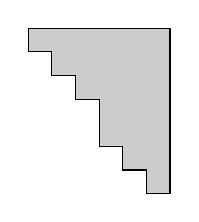
\begin{tikzpicture}[scale=0.3]
\fill[black!20] (0,0)--(0,-1)--(1,-1)--(1,-2)--(2,-2)--(2,-3)
    --(3,-3)--(3,-5)--(4,-5)--(4,-6)--(5,-6)--(5,-7)--(6,-7)--(6,0)--cycle;
\draw (0,0)--(0,-1)--(1,-1)--(1,-2)--(2,-2)--(2,-3)
    --(3,-3)--(3,-5)--(4,-5)--(4,-6)--(5,-6)--(5,-7)--(6,-7);
\draw[thin] (6,-7)--(6,0)--(0,0);
\end{tikzpicture}}\right)$$
where a cell is colored when it can contain a non-vanishing entry.
The top part of the matrix is then already echenolized, so that we
only have to re-echelonize the bottom right corner whose size is
the distance from the column corresponding to the erased variable
to the end. 
Thanks to the particular shape of the matrix, the echelonization can be 
performed efficiently: we combine the first rows (of the bottom right 
part) in order to clear the first unwanted nonzero entry and then 
proceed recursively.

\medskip

\noindent \textit{Updating a variable.}
%
Just like for creation, this happens when the program reaches an
affectation ``\verb?w = ...?'' where the variable \ttw is already 
defined.

This situation can actually be decomposed into three steps: first, we 
compute the right-hand-side and store it in a temporary variable \tttmp; 
second, we delete \ttw; third, we rename \tttmp in \ttw. The first step 
corresponds to the creation of a variable and was then already studied. 
Similarly, the second step is a variable deletion and again has already 
been discussed. As for the third step, it just changes the name of an
element of $\calV_t$ but does not affect the lattice $H_t$, nor the
matrix $M_t$.

\subsubsection{The case of \ZpLF.}

The way the package \ZpLF tracks precision is based on similar 
techniques but differs from \ZpLC in that it does not introduce a cap 
but instead allows $H_t$ to be a sub-$\Zp$-module of $E_t$ of any 
codimension.
This point of view is nice because it implies smaller objects and 
consequently leads to faster algorithms. However, it has a huge 
drawback; indeed, unlike lattices, submodules of $E_t$ of arbitrary 
codimensions are \emph{not} exact objects, in the sense that they cannot 
be represented by integral matrices in full generality. Consequently,
they cannot be encoded on a computer.
We work around this drawback by replacing everywhere exact $p$-adic 
numbers by Floating Point $p$-adic numbers (at some given precision) 
\cite{}.

The fact that the lattice $H_t$ can now have arbitrary codimension
translates to the fact the matrix $M_t$ can be rectangular.
Precisely, we will maintain matrices $M_t$ of the shape:
\begin{equation}
\label{eq:shapeM-ZpLF}
\left(\raisebox{-0.5\height}{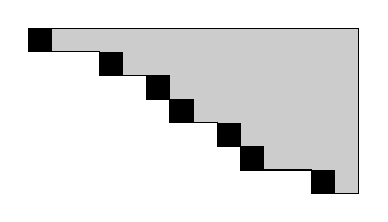
\begin{tikzpicture}[scale=0.3]
\fill[black!20] (0,0)--(0,-1)--(3,-1)--(3,-2)--(5,-2)--(5,-3)
    --(6,-3)--(6,-4)--(8,-4)--(8,-5)--(9,-5)--(9,-6)--(12,-6)
    --(12,-7)--(14,-7)--(14,0)--cycle;
\draw (0,0)--(0,-1)--(3,-1)--(3,-2)--(5,-2)--(5,-3)
    --(6,-3)--(6,-4)--(8,-4)--(8,-5)--(9,-5)--(9,-6)--(12,-6)
    --(12,-7)--(14,-7);
\fill (0,0) rectangle (1,-1);
\fill (3,-1) rectangle (4,-2);
\fill (5,-2) rectangle (6,-3);
\fill (6,-3) rectangle (7,-4);
\fill (8,-4) rectangle (9,-5);
\fill (9,-5) rectangle (10,-6);
\fill (12,-6) rectangle (13,-7);
\draw[thin] (14,-7)--(14,0)--(0,0);
\end{tikzpicture}}\right)
\end{equation}
where only the colored cells may contain a nonzero value and the 
black cells ---the so-called \emph{pivots}--- do not vanish. A
variable whose corresponding column contains a pivot will be called 
a \emph{pivot variable at time $t$}.

Below, we explain in more details how the package \ZpLF updates 
the matrix $M_t$ when a variable is created or deleted.

\medskip

\noindent \textit{Creating a variable.}
%
We assume first that the newly created variable is defined through an
affectation of the form:

\medskip

\hfill\verb?w = ?$f$\verb?(v_1,? \ldots\verb?, v_n)?\hfill\null

\medskip

\noindent
As already explained in the case of \ZpLC, this line of code is 
modeled by the mathematical mapping:
$$\begin{array}{rcl}
F: \quad E_t & \longrightarrow & E_{t+1} \smallskip \\
\underline x & \mapsto & \underline x \:\oplus f(x_1, \ldots, x_n).
\end{array}$$
Here $\underline x$ represents the state of memory at time $t$, 
and $x_i$ is the coordinate of $\underline x$ corresponding to the
variable $\ttv_i$.

In the \ZpLF framework, $H_{t+1}$ is defined as the image of $H_t$
under the differential $dF_{\underline x}$. Accordingly, the matrix
$M_{t+1}$ is defined as $M_{t+1} = \left(\begin{matrix}
M_t & C \end{matrix}\right)$
where $C$ is the column vector:
$$C = \sum_{i=1}^n \frac{\partial f}{\partial{\ttv_i}} (\underline x)
\cdot C_i.$$
However, we insist on the fact that all the above computations take
place in the ``ring'' of Floating Point $p$-adic numbers. Therefore,
we cannot guarantee that the rows of $M_{t+1}$ generate $H_{t+1}$.
Nonetheless, they generate a module which is expected to be closed 
to $H_{t+1}$.

\smallskip

If \ttw is created by the code
``\verb?w = ?\verb?R(?\text{value}\verb?, ?\text{prec}\verb?)?'',
we define $H_{t+1} = H_t \oplus p^{\text{prec}} \Zp e_\ttw$ and consequently:
$$M_{t+1} = \left(\begin{matrix}
M_t & 0 \smallskip \\ 0 & p^{\text{prec}}
\end{matrix}\right)$$
If $\text{prec}$ is $+\infty$ (or, equivalently, not specified), we
agree that $H_{t+1} = H_t$ and $M_{t+1} = (\begin{matrix} M_t & 0 
\end{matrix})$.

\medskip

\noindent \textit{Deleting a variable.} 
% 
As for \ZpLC, the matrix operation implied by the deletion of the 
variable \ttw is modeled by the deletion of the corresponding column 
of $M_t$. If \ttw is not a pivot variable at time $t$, the matrix 
$M_t$ keeps the form \eqref{eq:shapeM-ZpLF} after erasure; therefore
no more treatment is needed in this case.

Otherwise, we re-echelonize the matrix as follows. After the deletion 
of the column $C_\ttw$, we examine the first column $C$ which was 
located on the right of $C_\ttw$. Two situations may occur (depending
on the fact that $C$ was or was not a pivot column):

\noindent \hfill
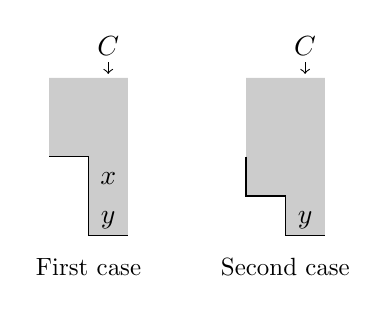
\begin{tikzpicture}[scale=0.5]
\fill[black!20] (0,0)--(1,0)--(1,-2)--(2,-2)--(2,2)--(0,2)--(0,0);
\draw (0,0)--(1,0)--(1,-2)--(2,-2);
\node at (1.5,2.8) { $C$ };
\draw[->] (1.5,2.4)--(1.5,2.1);
\node at (1.5,-0.5) { \ph $x$ };
\node at (1.5,-1.5) { \ph $y$ };
\node[scale=0.9] at (1,-2.8) { First case };
\begin{scope}[xshift=5cm]
\fill[black!20] (0,0)--(0,-1)--(1,-1)--(1,-2)--(2,-2)--(2,2)--(0,2)--(0,0);
\draw (0,0)--(0,-1)--(1,-1)--(1,-2)--(2,-2);
\node at (1.5,2.8) { $C$ };
\draw[->] (1.5,2.4)--(1.5,2.1);
\node at (1.5,-1.5) { \ph $y$ };
\node[scale=0.9] at (1,-2.8) { Second case };
\end{scope}
\end{tikzpicture}
\hfill\null

\noindent

In the first case, we perform row operations in order to replace the 
couple $(x,y)$ by $(d, 0)$ where $d$ is element of smallest valuation 
among $x$ and $y$. Observe that $y$ is necessarily nonzero in this case, 
so that $d$ does not vanish as well. After this operation, we move to
the next column and repeat the same process.

The second case is divided into two subcases. First, if $y$ does not 
vanish, it can serve as a pivot and the obtained matrix has the desired 
shape. When this occurs, the echelonization stops. On the contrary, if 
$y = 0$, we just untint the corresponding cell and move to the next 
column without modifying the matrix.

\subsection{Visualizing the precision}

Our package implements several methods giving access to the precision 
structure. In the subsection, we present and discuss the most relevant 
features in this direction.

\medskip

\noindent \textbf{Absolute precision of one element.}
%
This is the simplest accessible precision datum.
It is encapsulated in the notation when an element is printed. For
example, the (partial) session:

\smallskip

\noindent
\begin{tabular}{rl}
\cIn  & \verb?R = ZpLC(2, print_mode='digits')? \\
      & \verb?v = R(173,10); v? \\
\cOut & \verb?...0010101101?
\end{tabular}

\smallskip

\noindent
indicates that the absolute precision on \ttv is $10$ since
exactly $10$ digits are printed.
The method \verb?precision_absolute? provides a more easy-to-use
access to the absolute precision.

\smallskip

\noindent
\begin{tabular}{rl}
\cIn  & \verb?v.precision_absolute()? \\
\cOut & \verb?10?
\end{tabular}

\smallskip

\noindent

Both \ZpLC and \ZpLF compute the absolute precision of \ttv (at time 
$t$) as the smallest valuation of an entry of the column of $M_t$ 
corresponding to the variable \ttv. Alternatively, it can be defined as 
the unique integer $N$ for which $\pi_\ttv(H_t) = p^N \Zp$ where 
$\pi_\ttv : E_t \to \Qp$ takes a vector to its \ttv-coordinate.
This definition of the absolute precision sounds revelant because, if we 
believe that the submodule $H_t \subset E_t$ is supposed to encode the 
precision on the variables in $\calV_t$, 
Proposition~\ref{prop:precision} applied with the mapping $\pi_\ttv$ 
indicates that a good candidate for the precision on $e_\ttv$ is 
$\pi_\ttv(H_t) = p^N \Zp$.

\medskip

\noindent \textit{About correctness.}
%
We emphasize that the absolute precision computed this way is \emph{not} 
proved, either for \ZpLF or \ZpLC. However, in the case of \ZpLC, one
can be slightly more precise. Let $\calU_t$ be the vector space of 
user-defined variables before time $t$ and $U_t$ be the lattice
modeling the precision on them. The pair $(\calU_t, U_t)$ is defined 
inductively as follows: we set $\calU_0 = U_0 = 0$ and 
$\calU_{t+1} = \calU_t \oplus \Qp e_\ttw$,
$U_{t+1} = U_t \oplus p^{\text{prec}} \Zp e_\ttw$
when a new variable \ttw is created by
``\verb?w = R(?value\verb?, ?prec\verb?)?''; otherwise, we put 
$\calU_{t+1} = \calU_t$ and $U_{t+1} = U_t$. Moreover the values
entered by the user defines a vector (with integral coordinates)
$\underline u_t \in \calU_t$.

Similarly, in order to model the caps, we define a pair $(\calK_t, 
K_t)$ by the recurrence $\calK_{t+1} = \calK_t \oplus \Qp e_\ttw$,
$K_{t+1} = K_t \oplus p^{N_{t+1}} \Zp e_\ttw$
each time a new variable \ttw is created. 
Here, the exponent $N_{t+1}$ is the cap defined by Eq.~\eqref{eq:cap}.
In case of deletion, we put $\calK_{t+1} = \calK_t$ and $K_{t+1} = K_t$.

Taking the compositum of all the functions $\tilde F$ (\emph{cf} 
Eq.~\eqref{eq:tildeF}) from time $0$ to $t$, we find that the execution 
of the session until time $t$ is modeled by a mathematical function
$\Phi_t : \calU_t \oplus \calK_t \to E_t$.
From the design of \ZpLC, we deduce further that there exists a 
vector $\underline k_t \in K_t$ such that:
$$\Phi_t(\underline u_t \oplus \underline k_t) = \underline x_t 
\quad \text{and} \quad
d\Phi_t (U_t \oplus K_t) = H_t$$
where the differential of $\Phi_t$ is taken at the point
$\underline u_t \oplus \underline k_t$. 
Set $\Phi_{t,\ttv} = \pi_\ttv \circ \Phi_t$. It maps 
$\underline u_t \oplus \underline k_t$ to the \ttv-coordinate 
$x_{t,\ttv}$ of $\underline x_t$ and satisfies:
$$d\Phi_{t,\ttv} (U_t \oplus K_t) = \pi_\ttv(H_t) = p^N \Zp$$
where $N$ is the value returned by \verb?precision_absolute?. Thus, 
as soon as the assumptions of Proposition \ref{prop:precision} are
fulfilled, we derive
$\Phi_{t,\ttv} \big((\underline u_t + U_t) \oplus (\underline k_t + K_t)\big) = 
x_{t,\ttv} + p^N \Zp$.
Noting that $k_t \in K_t$, we finally get:
\begin{equation}
\label{eq:absprec}
\Phi_{t,\ttv} (\underline u_t + U_t) \subset
\Phi_{t,\ttv} \big((\underline u_t + U_t) \oplus K_t\big) = 
x_{t,\ttv} + p^N \Zp.
\end{equation}
The latter inclusion means that the computed value $x_{t,\ttv}$ is
accurate at precision $O(p^N)$, \emph{i.e.} that the output absolute
precision is correct. 

Unfortunately, checking automatically the assumptions of Proposition 
\ref{prop:precision} in full generality seems to be difficult, though it 
can be done by hand for many particular examples \cite{}.

\begin{rmk}
Assuming that Proposition \ref{prop:precision} applies, 
the absolute precision computed as above is optimal if and only if
the inclusion of \eqref{eq:absprec} is an equality. Applying again
Proposition \ref{prop:precision}
with the restricted mapping $\Phi_{t,\ttv} : \calU_t \to \Qp$ and the
lattice $U_t$, we find that this happens if and only if
$d\Phi_{t,\ttv}(U_t) = p^N \Zp$.

Unfortunately, the latter condition cannot be checked on the matrix 
$M_t$ (because of reductions). 
However it is possible (and easy) to check whether the weaker condition 
$d\Phi_{t,\ttv}(K_t) \subsetneq p^N \Zp$. This checking is achieved by 
the method
\verb?is_precision_capped? (provided by our package) which returns true 
if $d\Phi_{t,\ttv}(K_t) = p^N \Zp$. As a consequence, when this method
answers false, the absolute precision computed by the software is
likely optimal.
\end{rmk}

\noindent \textbf{Precision on a subset of elements.}

\medskip

\noindent \textit{Diffused digits of precision.}

\subsection{Complexity}

We now discuss the cost of the above operations.
For this,
it is convenient to introduce a total order on $\calV_t$: for $\ttv, 
\ttw \in \calV_t$, we convene that $\ttv <_t \ttw$ is \ttv was created 
before~\ttw. By construction, the columns of the matrix $M_t$ are 
ordered with respect to $<_t$.
For $\ttv \in \calV_t$, we define the \emph{index} of \ttv, denoted by 
$\ind_t(\ttv)$ as the number of elements of $\calV_t$ which are not 
greater than \ttv. If we sort the elements of $\calV_t$ by increasing 
order, \ttv then appears in $\ind_t(\ttv)$-th position.
We also define the \emph{coindex} of \ttv by
$\coind_t(\ttv) = \card \calV_t - \ind_t(\ttv)$.

\medskip

\noindent \textbf{Creating a variable.}

\ZpLC: $O\bigg(\sum_{i=1}^n \ind_t(\ttv_i)\bigg) \subset 
O\big(n \cdot \card \calV_t\big)$

\ZpLF: 

\medskip

\noindent \textit{Deleting a variable.}

$$O\big(\coind_t(\ttw)^2\big)$$

\medskip

\noindent \textit{Temporal locality.}

\medskip

\noindent \textbf{Correctness.}

\subsubsection*{Tracking precision}

\subsubsection*{Complexity}

\section{More examples}

\begin{tabular}{|l|l|}
\verb?R = Zp(2)? & \verb?R = ZpL(2)? \\
\multicolumn{2}{|l|}{\tt x, y, z, t = R(1,15), R(1,15), R(1,15), R(3,15)} \\
\multicolumn{2}{|l|}{\tt for \_ in range(20):} \\
\multicolumn{2}{|l|}{\tt \ \ \ \ x, y, z, t = y, z, t, (y*t + z*z)/x} \\
\multicolumn{2}{|l|}{\tt \ \ \ \ print t} \\
\hfill\verb?...000000000000100? & \hfill\verb?...000000000000100? \\
\hfill\verb?...000000000001101? & \hfill\verb?...000000000001101? \\
\hfill\verb?...000000000110111? & \hfill\verb?...000000000110111? \\
\hfill\verb?...101010111010111? & \hfill\verb?...101010111010111? \\
\hfill\verb?...1100111101111? & \hfill\verb?...101100111101111? \\
\hfill\verb?...1110000010010? & \hfill\verb?...111110000010010? \\
\hfill\verb?...0001000111001? & \hfill\verb?...100001000111001? \\
\hfill\verb?...0000011111101? & \hfill\verb?...100000011111101? \\
\hfill\verb?...1000000110101? & \hfill\verb?...001000000110101? \\
\hfill\verb?...101101010011? & \hfill\verb?...010101101010011? \\
\hfill\verb?...110000000000? & \hfill\verb?...001110000000000? \\
\hfill\verb?...000101011101? & \hfill\verb?...111000101011101? \\
\hfill\verb?...001001101011? & \hfill\verb?...111001001101011? \\
\hfill\verb?...000011110011? & \hfill\verb?...111000011110011? \\
\hfill\verb?...11? & \hfill\verb?...0000000111? \\
\hfill\verb?...10? & \hfill\verb?...1010001110? \\
\hfill\verb?...01? & \hfill\verb?...1110110001? \\
\hfill\verb?...01? & \hfill\verb?...011110111001? \\
\hfill\verb?...01? & \hfill\verb?...100101101001001? \\
\hfill\verb?...1? & \hfill\verb?...11111000011? \\
\end{tabular}

\begin{itemize}
\item SOMOS sequence
\item many multiplications of matrices
\item Dodgson algorithm
\item subresultants
\item Grobner basis
\item $p$-adic differential equations
\end{itemize}

\subsubsection{$p$-adic differential equations}


In \cite{LV16}, the behaviour of the precision when solving
$p$-adic differential equations with separation of 
variables has been studied.
The authors have investigated the gap when that appears
when applying a Newton-method solver between
the theoretic loss in precision and the 
actual loss in precision for a naive implemenationin \verb?Zp(p)?.
We can reach this theoretical loss in precision using \verb?ZpL?.
We use a generic \verb?Newton_Iteration_Solver(g,h,N)?
that applies \verb?N? steps of the Newton method for 
$y'=g \times h(y)$ as described in \citep{LV16}. 

\begin{tabular}{|l|l|}
\verb?R = Qp(2,250)? & \verb?R = QpL(2,250)? \\
\verb?S = Zp(2,250)? & \verb?S = ZpL(2,250)? \\
\multicolumn{2}{|l|}{\tt A.<x> = PowerSeriesRing(R,32) } \\
\multicolumn{2}{|l|}{\tt B.<x> = PowerSeriesRing(S,32)) } \\
\multicolumn{2}{|l|}{\tt h,y =1+x+x\^{}3 , x+x\^{}2*A(B.random\_element()) } \\
\multicolumn{2}{|l|}{\tt g=y.derivative()/h(y) } \\
\multicolumn{2}{|l|}{\tt s=Newton\_Iteration\_Solver(g,h,5)} \\
\multicolumn{2}{|l|}{\tt print 250-(s[31].lift()-y[31].lift()).valuation(2)} \\
\hfill\verb?9? & \hfill\verb?4? \\
\end{tabular}
The last line provides the loss in precision between the
original solution of the differential equation and its approximation
obtained through computation.
The theorical loss in precision for the coefficient of $t^{31}$
is $\lfloor log_2 (31)\rfloor=4$ and is then reached, whereas the
loss in precision for a naive implementation is clearly more severe.


\section{Conclusion}

\begin{itemize}
\item In which case should we use this package? Mainly for exploration
\item example of $p$-adic differential equations (especially for $p=2$)
\end{itemize}

\subsection{Exploration}

The purpose of this package is that of exploration
of the $p$-adic precision.
We conclude with a last example coming
from the field of the computation of
isogenies between elliptic curves over finite fields.
Techniques to compute these isogenies
through the solving of $p$-adic differential equations
have a long history, and a first
analysis of the behaviour of precision using
lattices has been investigated in \cite{LV16}.

In that article, the authors were interested in
solving $y'^2=g \times h(y)$ with
$g,h,y \in \mathbb{Z}_p \llbracket x \rrbracket$
such that $g(0)=h(0)=1$ and $y(0)=0.$

The main result was that the intrinsic loss in precision
when computing the coefficient $x^n$ of $y$
from $g$ and $h$ was in $\log_p(n)$
even though a naive analysis of
the Newton method for solving the equation
yield a loss in $\log_p(n)^2.$

However, this does not encompass the case of 
elliptic curves defined and isogeneous 
over $\mathbb{Q},$ which can yield a differential 
equation with a solution $y$ whose coefficients
have negative valuation.

For instance, the curves 
$E: \: y^2=x^3+1$
and $E': \: y^2=+ (m^2-1)x^2/4 + m^6$ are isogeneous
over $\mathbb{Q}$ if  $m$ is an odd integer.
We take $m=67.$ The corresponding isogeny has coefficients with possibly
negative $3$-adic valuation.

We can solve numerically 
the corresponding differential equation
using the algorithm of \cite{Lercier-Sirvent:08}
over $\mathbb{Q}_3$ with lattice precision.
We use an initial precision of 50 digits.
Any generic implementation of the Newton
method of \cite{Lercier-Sirvent:08} is enough.

\begin{tabular}{|l|}
\verb?    R = QpL(3,50)? \\
\verb?    A.<x> = PolynomialRing(R)?\\
\verb?    m=67?\\
\verb?    g=1+(1/4)*x^2+x^6?\\
\verb?    h=1+((m^2)/4)*x^2+m^6* x^6?\\
\verb?    y=Lercier_Sirvent(g,h,64)?\\
\verb?    y[31]?\\
\verb?(467995903278061284942799/3^14 + O(3^36))*x^31?\\
\end{tabular}

We can then see that up to $63,$ the behaviour
of the loss in relative precision is the same
as for the coefficient in $x^{31}$: \textbf{no loss
occured}.
Thus, those simple manipulations
hint at a different behaviour for the loss 
in precision in at least some special cases of
of isogenies defined over $\mathbb{Q}$
but not necessarily over $\mathbb{Z}_p.$ 

\bibliographystyle{plain}
\bibliography{ZpL}


\end{document}

